% =============================================================================
%  RISE Talk: Connecting the Dots — Barrier Synthesis for Python
%  PRESENTER DECK (beautiful, visual, minimal text)
% =============================================================================
\documentclass[aspectratio=169]{beamer}
\usetheme{metropolis}
\usepackage{appendixnumberbeamer}
\usepackage{amsmath,amssymb}
\usepackage{tikz}
\usetikzlibrary{arrows.meta,positioning,shapes.geometric,calc,decorations.pathmorphing,backgrounds,fit}
\usepackage{listings}
\usepackage{booktabs}
\usepackage{xcolor}
\usepackage{fontawesome5}

% ── Color palette ────────────────────────────────────────────────────────────
\definecolor{accent}{HTML}{2563EB}
\definecolor{accentdark}{HTML}{1E40AF}
\definecolor{safe}{HTML}{059669}
\definecolor{unsafe}{HTML}{DC2626}
\definecolor{warn}{HTML}{D97706}
\definecolor{bg}{HTML}{F8FAFC}
\definecolor{codebg}{HTML}{F1F5F9}
\definecolor{hilbert}{HTML}{7C3AED}    % violet
\definecolor{control}{HTML}{EC4899}    % pink
\definecolor{verify}{HTML}{0891B2}     % cyan
\definecolor{steal}{HTML}{F59E0B}      % amber
\definecolor{ship}{HTML}{059669}       % green

\setbeamercolor{frametitle}{bg=accent,fg=white}
\setbeamercolor{progress bar}{fg=accent}
\setbeamercolor{alerted text}{fg=unsafe}

\lstset{
  basicstyle=\ttfamily\scriptsize,
  breaklines=true, frame=none,
  backgroundcolor=\color{codebg},
  keywordstyle=\color{accentdark}\bfseries,
  commentstyle=\color{safe!80!black},
  stringstyle=\color{unsafe!80!black},
  showstringspaces=false,
}

\title{\textbf{Connecting the Dots}}
\subtitle{From Hilbert's 17th Problem to a Python bug finder}
\author{}
\date{RISE}
\setbeamertemplate{navigation symbols}{}

\begin{document}

% ═══════════════════════════════════════════════════════════════════════════
%  TITLE
% ═══════════════════════════════════════════════════════════════════════════

\begin{frame}[plain]
\titlepage
\end{frame}

% ═══════════════════════════════════════════════════════════════════════════
%  OPENING — THE QUESTION
% ═══════════════════════════════════════════════════════════════════════════

\begin{frame}{The Prompt That Started Everything}
\begin{center}
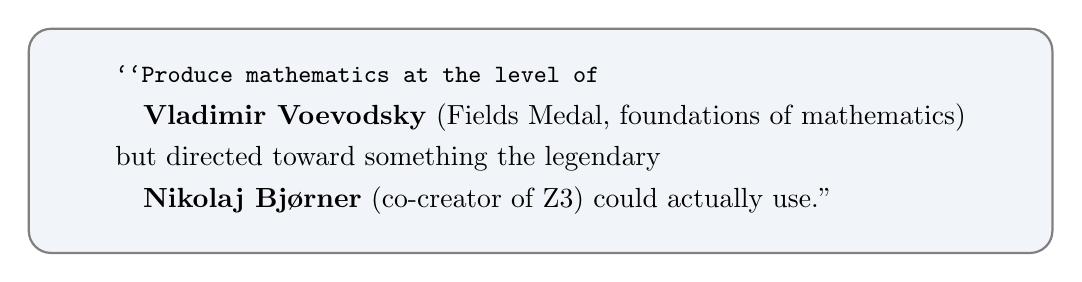
\begin{tikzpicture}
  \node[draw, rounded corners=8pt, fill=codebg, thick, draw=gray, minimum width=13cm, align=left, inner sep=14pt] {
    \small\ttfamily
    ``Produce mathematics at the level of\\[3pt]
    \hspace{1em}\textbf{Vladimir Voevodsky} (Fields Medal, foundations of mathematics)\\[3pt]
    but directed toward something the legendary\\[3pt]
    \hspace{1em}\textbf{Nikolaj Bj\o rner} (co-creator of Z3) could actually use.''
  };
\end{tikzpicture}
\end{center}

\vspace{0.8em}
\begin{columns}[c]
\begin{column}{0.45\textwidth}
\centering
\textcolor{hilbert}{\textbf{Voevodsky}}\\
\small Fields Medal 2002\\Homotopy type theory\\Proof = computation\\
\textit{Foundation-shaking math}
\end{column}
\begin{column}{0.1\textwidth}
\centering\Large\textcolor{gray}{$\times$}
\end{column}
\begin{column}{0.45\textwidth}
\centering
\textcolor{verify}{\textbf{Bj\o rner}}\\
\small Co-creator of Z3\\SMT solving at scale\\Proof = solver output\\
\textit{Industrial verification}
\end{column}
\end{columns}

\vspace{0.8em}
\centering
The AI generated dozens of ideas. Most were slop.\\[4pt]
\textbf{One thread survived.}
\end{frame}

% ═══════════════════════════════════════════════════════════════════════════
%  ACT I — THE DOTS
% ═══════════════════════════════════════════════════════════════════════════

\begin{frame}{Five ``Random'' Dots}
\begin{center}

\begin{tikzpicture}[
  dot/.style={circle, minimum size=12mm, draw=none, font=\footnotesize\bfseries, text=white}
]
  \node[dot, fill=hilbert] (d1) at (0,0) {1900};
  \node[dot, fill=hilbert!70] (d2) at (3,0) {1974};
  \node[dot, fill=control] (d3) at (6,0) {2000};
  \node[dot, fill=verify] (d4) at (9,0) {2004};
  \node[dot, fill=steal] (d5) at (12,0) {\faTools};

  \node[below=5mm, font=\scriptsize, text=hilbert, align=center] at (d1) {Hilbert's\\17th Problem};
  \node[below=5mm, font=\scriptsize, text=hilbert!70, align=center] at (d2) {Stengle's\\Positivstellensatz};
  \node[below=5mm, font=\scriptsize, text=control, align=center] at (d3) {Parrilo's SOS\\(control theory)};
  \node[below=5mm, font=\scriptsize, text=verify, align=center] at (d4) {Prajna's barriers\\(ctrl $\to$ verif.)};
  \node[below=5mm, font=\scriptsize, text=steal, align=center] at (d5) {20 techniques\\we stole};
\end{tikzpicture}
\end{center}

\vspace{1em}
\centering
Pure math $\to$ real algebraic geometry $\to$ control theory $\to$ verification $\to$ \textbf{Python}\\[4pt]
\small\textit{Each jump looked unreasonable at the time.}
\end{frame}

% ── Dot 1: Hilbert ──────────────────────────────────────────────────────────

\begin{frame}{Dot 1: Hilbert's 17th Problem (1900)}
\begin{columns}[c]
\begin{column}{0.58\textwidth}
\begin{quote}
\large\textit{``Is every non-negative polynomial\\a sum of squares of rational functions?''}
\end{quote}
\vspace{0.5em}
\begin{itemize}
  \item Posed at the 1900 International Congress
  \item Answered \textbf{yes} by Artin (1927)
  \item A non-negative polynomial $p(x) \ge 0$ can be certified by decomposing it into $\sum q_i^2$
  \item \textbf{No one was thinking about software}
\end{itemize}
\end{column}
\begin{column}{0.38\textwidth}
\centering
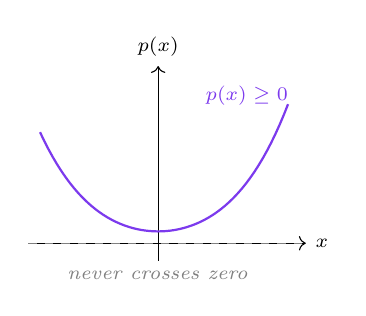
\begin{tikzpicture}[scale=0.75]
  \draw[->] (-2.2,0) -- (2.5,0) node[right,font=\scriptsize]{$x$};
  \draw[->] (0,-0.3) -- (0,3) node[above,font=\scriptsize]{$p(x)$};
  \draw[thick, hilbert, domain=-2:2.2, samples=60] plot (\x, {0.3*\x*\x + 0.1*\x*\x*\x*\x*0.3 + 0.2});
  \node[font=\scriptsize, hilbert] at (1.5, 2.5) {$p(x) \ge 0$};
  \draw[dashed, gray] (-2.2,0) -- (2.5,0);
  \node[font=\scriptsize, gray, below] at (0,-0.3) {\textit{never crosses zero}};
\end{tikzpicture}
\end{column}
\end{columns}
\end{frame}

% ── Dot 2: Stengle ─────────────────────────────────────────────────────────

\begin{frame}{Dot 2: Stengle's Positivstellensatz (1974)}
\begin{center}
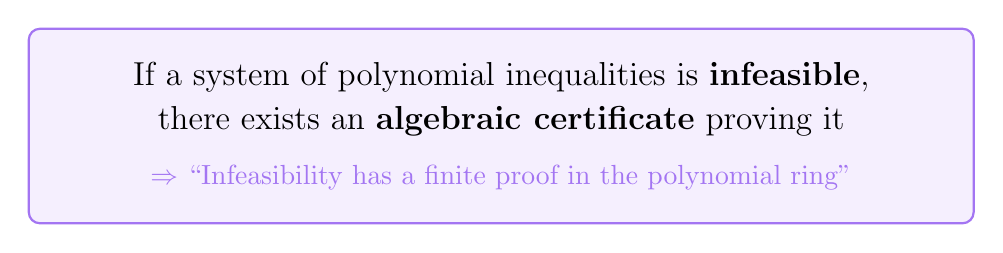
\begin{tikzpicture}
  \node[draw, rounded corners, fill=hilbert!8, thick, draw=hilbert!70, minimum width=12cm, align=center, inner sep=12pt] {
    \large If a system of polynomial inequalities is \textbf{infeasible},\\[4pt]
    \large there exists an \textbf{algebraic certificate} proving it\\[8pt]
    \normalsize\textcolor{hilbert!70}{$\Rightarrow$ ``Infeasibility has a finite proof in the polynomial ring''}
  };
\end{tikzpicture}
\end{center}

\vspace{1em}
\begin{itemize}
  \item Generalizes Hilbert--Artin to \textbf{semialgebraic sets} (regions defined by polynomial $\ge$, $=$, $\le$)
  \item If two regions don't overlap, you can \emph{prove} it with a polynomial identity
  \item Still pure math. No computers, no programs, no control systems.
\end{itemize}

\vspace{0.5em}
\centering
\textcolor{hilbert!70}{\faLightbulb}\; \textbf{Key insight we'll use:} if safe $\cap$ unsafe $= \varnothing$, a polynomial \emph{fence} must exist.
\end{frame}

% ── Dot 3: Parrilo / SOS / Control Theory ──────────────────────────────────

\begin{frame}{Dot 3: Parrilo's SOS Programming (2000)}
\begin{center}
\large The jump to \textbf{control theory}
\end{center}

\vspace{0.5em}
\begin{columns}[c]
\begin{column}{0.55\textwidth}
\begin{itemize}
  \item \textbf{Problem:} control engineers need to prove robots / aircraft / reactors \textbf{stay safe}
  \item Lyapunov stability: find a function $V(x)$ that proves the system never leaves a safe region
  \item Parrilo: checking ``$p(x) \ge 0$'' is equivalent to a \textbf{semidefinite program} (SDP)
  \item \textbf{Suddenly computable}
\end{itemize}
\end{column}
\begin{column}{0.4\textwidth}
\centering
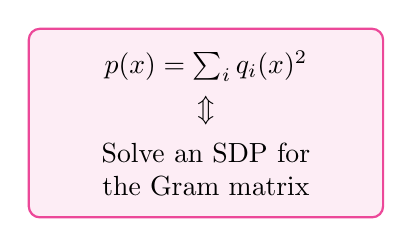
\begin{tikzpicture}
  \node[draw, rounded corners, fill=control!10, thick, draw=control, minimum width=4.5cm, align=center, inner sep=8pt] {
    $p(x) = \sum_i q_i(x)^2$\\[4pt]
    $\Updownarrow$\\[4pt]
    Solve an SDP for\\
    the Gram matrix
  };
\end{tikzpicture}
\end{column}
\end{columns}

\vspace{0.8em}
\centering
\textcolor{control}{\faLightbulb}\; Hilbert's 1900 question $\to$ a \textbf{tractable optimization problem} in 2000.
\end{frame}

% ── Dot 4: Prajna / Barrier Certificates ───────────────────────────────────

\begin{frame}{Dot 4: Prajna's Barrier Certificates (HSCC 2004)}
\begin{center}
\large The jump from \textbf{control theory} to \textbf{verification}
\end{center}

\vspace{0.5em}
\begin{center}
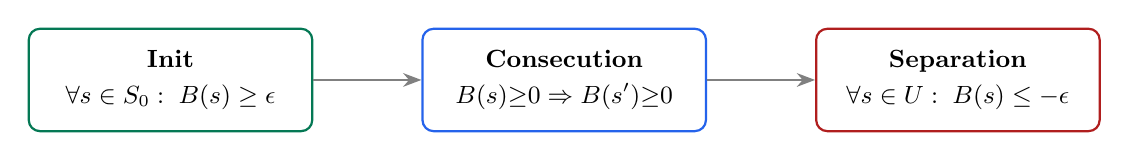
\begin{tikzpicture}[
  obl/.style={draw, rounded corners, fill=white, minimum width=3.6cm, minimum height=1.3cm, align=center, font=\small, thick}
]
  \node[obl, draw=safe!80!black] (init) at (0,0) {
    \textbf{Init}\\[2pt]
    $\forall s \in S_0:\; B(s) \ge \epsilon$
  };
  \node[obl, draw=accent] (cons) at (5,0) {
    \textbf{Consecution}\\[2pt]
    $B(s){\ge}0 \Rightarrow B(s'){\ge}0$
  };
  \node[obl, draw=unsafe!80!black] (sep) at (10,0) {
    \textbf{Separation}\\[2pt]
    $\forall s \in U:\; B(s) \le -\epsilon$
  };

  \draw[-{Stealth}, thick, gray] (init) -- (cons);
  \draw[-{Stealth}, thick, gray] (cons) -- (sep);
\end{tikzpicture}
\end{center}

\vspace{0.5em}
\begin{itemize}
  \item Prajna \& Jadbabaie: use barrier functions to prove \textbf{safety}, not just stability
  \item Three obligations. If all hold, unsafe states are \textbf{provably unreachable}.
  \item Originally for continuous dynamical systems (robots, circuits).
\end{itemize}

\centering
\textcolor{verify}{\faLightbulb}\; We use this \textbf{verbatim} --- over Python bytecode state.
\end{frame}

% ── Dot 5: The Theft ──────────────────────────────────────────────────────

\begin{frame}{Dot 5: The 20 Techniques We Stole}
\begin{center}
\large With the barrier \textbf{interface} in hand,\\[4pt]
\normalsize every verification technique becomes a \textbf{specialized solver}\\for one or more of the three obligations.
\end{center}

\vspace{0.8em}
\begin{center}
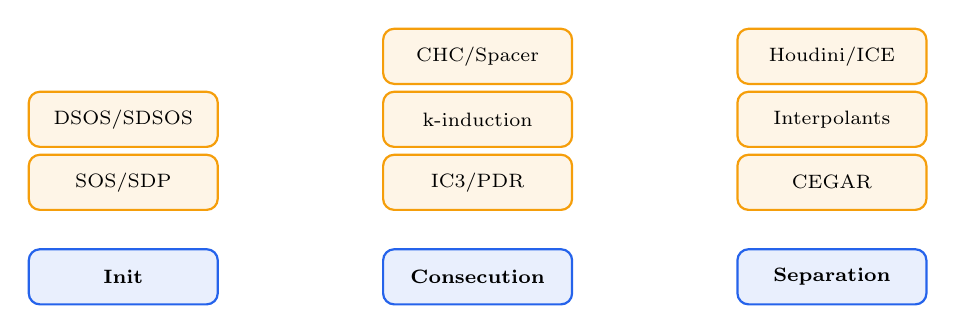
\begin{tikzpicture}[
  method/.style={draw, rounded corners, fill=steal!10, minimum width=2.4cm, minimum height=0.7cm, align=center, font=\scriptsize, thick, draw=steal},
  obl/.style={draw, rounded corners, fill=accent!10, minimum width=2.4cm, minimum height=0.7cm, align=center, font=\scriptsize\bfseries, thick, draw=accent}
]
  \node[obl] (init) at (0,0) {Init};
  \node[obl] (cons) at (4.5,0) {Consecution};
  \node[obl] (sep) at (9,0) {Separation};

  \node[method] at (0,1.2)   {SOS/SDP};
  \node[method] at (0,2.0)   {DSOS/SDSOS};

  \node[method] at (4.5,1.2) {IC3/PDR};
  \node[method] at (4.5,2.0) {k-induction};
  \node[method] at (4.5,2.8) {CHC/Spacer};

  \node[method] at (9,1.2)   {CEGAR};
  \node[method] at (9,2.0)   {Interpolants};
  \node[method] at (9,2.8)   {Houdini/ICE};
\end{tikzpicture}
\end{center}

\vspace{0.3em}
\centering\small
Every paper answers one question about $B$. Composition is \textbf{coherent}, not eclectic.
\end{frame}

% ── Connecting ─────────────────────────────────────────────────────────────

\begin{frame}{Connecting the Dots}
\begin{center}
\begin{tikzpicture}[
  dot/.style={circle, minimum size=11mm, draw=none, font=\small\bfseries, text=white},
  conn/.style={-{Stealth[length=3mm]}, very thick}
]
  \node[dot, fill=hilbert] (d1) at (0,0) {H17};
  \node[dot, fill=hilbert!70] (d2) at (3,0) {Sten};
  \node[dot, fill=control] (d3) at (6,0) {SOS};
  \node[dot, fill=verify] (d4) at (9,0) {$B$};
  \node[dot, fill=steal] (d5) at (12,0) {\faTools};

  \draw[conn, hilbert!50] (d1) -- (d2);
  \draw[conn, control!50] (d2) -- (d3);
  \draw[conn, verify!50] (d3) -- (d4);
  \draw[conn, steal!50] (d4) -- (d5);

  \node[below=6mm, font=\scriptsize, align=center] at (1.5,0) {\textit{pure math}\\$\to$ \textit{certificates}};
  \node[below=6mm, font=\scriptsize, align=center] at (4.5,0) {\textit{certificates}\\$\to$ \textit{computable}};
  \node[below=6mm, font=\scriptsize, align=center] at (7.5,0) {\textit{control}\\$\to$ \textit{verification}};
  \node[below=6mm, font=\scriptsize, align=center] at (10.5,0) {\textit{interface}\\$\to$ \textit{portfolio}};
\end{tikzpicture}
\end{center}

\vspace{1em}
\begin{center}
\large \textbf{126 years of seemingly unrelated work.}\\[6pt]
\normalsize Each dot looked like a different field entirely.\\
Together they form a \textbf{complete Python bug-finding pipeline}.
\end{center}
\end{frame}

% ═══════════════════════════════════════════════════════════════════════════
%  ACT II — WHY BARRIER THEORY
% ═══════════════════════════════════════════════════════════════════════════

\begin{frame}{Why a New Theoretical Basis?}
\begin{center}
\large Existing verification methods work. Why didn't we just \emph{use} them?
\end{center}

\vspace{0.8em}
\begin{columns}[T]
\begin{column}{0.48\textwidth}
\textbf{What existing methods give you:}
\begin{itemize}
  \item Abstract interpretation: sound, but \textbf{no composition API} across techniques
  \item Model checking: precise, but \textbf{state explosion} for numeric programs
  \item SMT alone: powerful, but \textbf{no structured proof artifact} you can audit
  \item Each method works in isolation; combining them is ad hoc
\end{itemize}
\end{column}
\begin{column}{0.48\textwidth}
\textbf{What barrier theory adds:}
\begin{itemize}
  \item \textbf{Three universal obligations} that any method can discharge
  \item Methods \textbf{compose} because they all serve the same $B$
  \item Failure is \textbf{informative}: obligation counterexamples route to the next method
  \item Every decision maps to an \textbf{auditable proof object}
  \item A shared interface turns a paper zoo into a \textbf{coherent portfolio}
\end{itemize}
\end{column}
\end{columns}

\vspace{0.5em}
\centering
\textit{Barrier theory isn't one more method. It's the \textbf{interface} that lets all methods cooperate.}
\end{frame}

\begin{frame}{The Unifying Interface}
\begin{center}
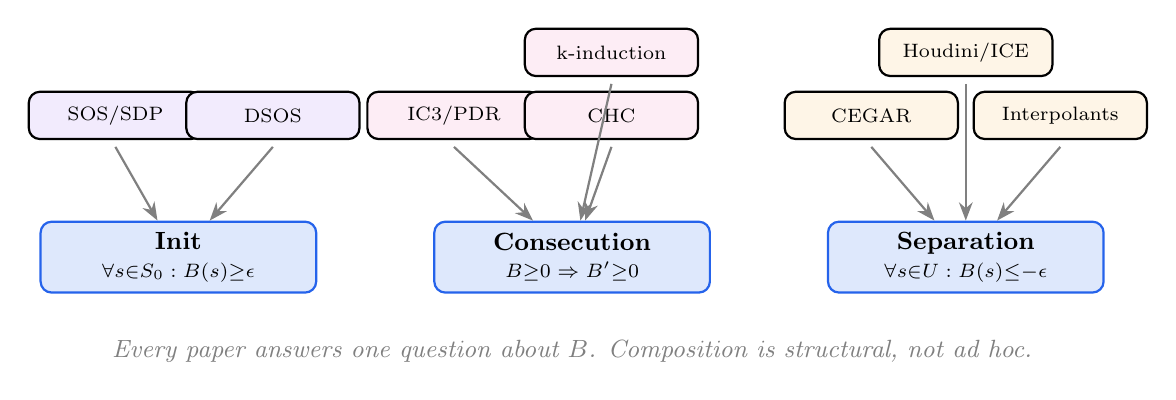
\begin{tikzpicture}[
  method/.style={draw, rounded corners, fill=bg, minimum width=2.2cm, minimum height=0.6cm, align=center, font=\scriptsize, thick},
  obl/.style={draw, rounded corners, fill=accent!15, minimum width=3.5cm, minimum height=0.9cm, align=center, font=\small\bfseries, thick, draw=accent}
]
  % Obligations
  \node[obl] (init) at (0,-0.3) {Init\\[-1pt]\scriptsize$\forall s{\in}S_0: B(s){\ge}\epsilon$};
  \node[obl] (cons) at (5,-0.3) {Consecution\\[-1pt]\scriptsize$B{\ge}0 \Rightarrow B'{\ge}0$};
  \node[obl] (sep) at (10,-0.3) {Separation\\[-1pt]\scriptsize$\forall s{\in}U: B(s){\le}{-}\epsilon$};

  % Methods feeding in
  \node[method, fill=hilbert!10] at (-0.8,1.5) {SOS/SDP};
  \node[method, fill=hilbert!10] at (1.2,1.5) {DSOS};
  \draw[-{Stealth}, gray, thick] (-0.8,1.1) -- (init);
  \draw[-{Stealth}, gray, thick] (1.2,1.1) -- (init);

  \node[method, fill=control!10] at (3.5,1.5) {IC3/PDR};
  \node[method, fill=control!10] at (5.5,1.5) {CHC};
  \node[method, fill=control!10] at (5.5,2.3) {k-induction};
  \draw[-{Stealth}, gray, thick] (3.5,1.1) -- (cons);
  \draw[-{Stealth}, gray, thick] (5.5,1.1) -- (cons);
  \draw[-{Stealth}, gray, thick] (5.5,1.9) -- (cons);

  \node[method, fill=steal!10] at (8.8,1.5) {CEGAR};
  \node[method, fill=steal!10] at (11.2,1.5) {Interpolants};
  \node[method, fill=steal!10] at (10,2.3) {Houdini/ICE};
  \draw[-{Stealth}, gray, thick] (8.8,1.1) -- (sep);
  \draw[-{Stealth}, gray, thick] (11.2,1.1) -- (sep);
  \draw[-{Stealth}, gray, thick] (10,1.9) -- (sep);

  % Label
  \node[font=\small\itshape, text=gray] at (5,-1.5) {Every paper answers one question about $B$. Composition is structural, not ad hoc.};
\end{tikzpicture}
\end{center}
\end{frame}

\begin{frame}{Why Barriers Beat the Status Quo}
\begin{columns}[T]
\begin{column}{0.31\textwidth}
\begin{block}{\textcolor{unsafe}{Linters}}
\begin{itemize}
  \item Fast, no proofs
  \item Can't reason about paths
  \item 80--95\% false positives
  \item $\to$ alert fatigue
\end{itemize}
\end{block}
\end{column}
\begin{column}{0.31\textwidth}
\begin{block}{\textcolor{warn}{Testing/fuzzing}}
\begin{itemize}
  \item Finds bugs, never proves absence
  \item $2^{64}$ inputs
  \item Can't close issues as ``safe''
  \item Expensive
\end{itemize}
\end{block}
\end{column}
\begin{column}{0.31\textwidth}
\begin{block}{\textcolor{safe}{Barrier certs}}
\begin{itemize}
  \item \textbf{Mathematical proof}
  \item Path-sensitive
  \item Handles loops
  \item \textbf{Eliminates silently}
\end{itemize}
\end{block}
\end{column}
\end{columns}

\vspace{0.8em}
\centering
On real repos: \textbf{99\% of candidate bugs proven unreachable.}\\
Only $\sim$1\% survive for triage.
\end{frame}

\begin{frame}{Proof, Not Confidence}
\begin{center}
\renewcommand{\arraystretch}{1.5}
\begin{tabular}{l@{\hspace{2em}}ccc}
\toprule
& \textbf{Linter} & \textbf{LLM triage} & \textbf{Barrier cert.} \\
\midrule
Proves absence       & \textcolor{unsafe}{\faTimes} & \textcolor{unsafe}{\faTimes} & \textcolor{safe}{\faCheck} \\
Auditable artifact   & \textcolor{unsafe}{\faTimes} & \textcolor{warn}{$\sim$} & \textcolor{safe}{\faCheck} \\
Path-sensitive       & \textcolor{unsafe}{\faTimes} & \textcolor{warn}{$\sim$} & \textcolor{safe}{\faCheck} \\
Handles loops        & \textcolor{unsafe}{\faTimes} & \textcolor{unsafe}{\faTimes} & \textcolor{safe}{\faCheck} \\
Scales to CI         & \textcolor{safe}{\faCheck} & \textcolor{warn}{$\sim$} & \textcolor{safe}{\faCheck} \\
\bottomrule
\end{tabular}
\end{center}

\vspace{0.8em}
\centering
A barrier certificate is a \textbf{proof object}: template + coefficients + checked obligations + site metadata.\\
You can audit it. You can replay it. It doesn't hallucinate.
\end{frame}

% ═══════════════════════════════════════════════════════════════════════════
%  ACT III — CONCRETE EXAMPLE
% ═══════════════════════════════════════════════════════════════════════════

\begin{frame}[fragile]{Concrete Example: DIV\_ZERO with a Polynomial Barrier}
\begin{columns}[T]
\begin{column}{0.44\textwidth}
\begin{lstlisting}[language=Python]
def safe_divide(a, b):
    if b != 0:
        return a / b  # safe?
    return 0.0
\end{lstlisting}

\vspace{0.5em}
\textbf{State variable:} $x = \texttt{b}$\\[3pt]
\textbf{Unsafe set:} $U = \{x : x = 0\}$\\[3pt]
\textbf{Guard:} division reached only when $x \neq 0$
\end{column}
\begin{column}{0.52\textwidth}
\begin{block}{Choose barrier: $B(x) = x - \tfrac{1}{2}$}
\end{block}

\vspace{0.3em}
\textbf{Check three obligations:}
\begin{enumerate}
  \item \textcolor{safe}{\faCheck}\; \textbf{Init:} after guard, $|x| \ge 1$ (integers)\\$\Rightarrow B(x) \ge \tfrac{1}{2} > 0$
  \item \textcolor{safe}{\faCheck}\; \textbf{Consecution:} $x$ is unchanged on the path to division
  \item \textcolor{safe}{\faCheck}\; \textbf{Separation:} $B(0) = -\tfrac{1}{2} < 0$
\end{enumerate}

\vspace{0.5em}
$\Rightarrow$ \textbf{DIV\_ZERO is unreachable.}\\
\textit{Proven by Hilbert $\to$ Stengle $\to$ Parrilo $\to$ Prajna.}
\end{column}
\end{columns}
\end{frame}

\begin{frame}{The Polynomial Fence, Visually}
\begin{center}
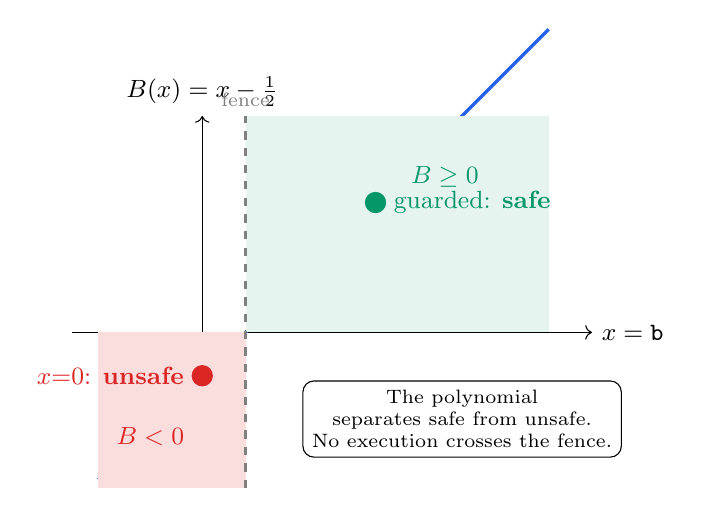
\begin{tikzpicture}[scale=1.1]
  % axes
  \draw[->] (-1.5,0) -- (4.5,0) node[right,font=\small]{$x = \texttt{b}$};
  \draw[->] (0,-1.8) -- (0,2.5) node[above,font=\small]{$B(x) = x - \tfrac{1}{2}$};

  % barrier line
  \draw[very thick, accent, domain=-1.2:4, samples=50] plot (\x, {\x - 0.5});

  % unsafe region
  \fill[unsafe!15] (-1.2,-1.8) rectangle (0.5,0);
  \node[font=\small, unsafe] at (-0.6, -1.2) {$B < 0$};

  % safe region
  \fill[safe!10] (0.5,0) rectangle (4,2.5);
  \node[font=\small, safe] at (2.8, 1.8) {$B \ge 0$};

  % zero crossing
  \draw[dashed, gray, thick] (0.5,-1.8) -- (0.5,2.5);
  \node[font=\scriptsize, gray, above] at (0.5,2.5) {fence};

  % unsafe point
  \fill[unsafe] (0,-0.5) circle (3.5pt);
  \node[font=\small, unsafe, left] at (-0.1,-0.5) {$x{=}0$: \textbf{unsafe}};

  % safe point
  \fill[safe] (2,1.5) circle (3.5pt);
  \node[font=\small, safe, right] at (2.1,1.5) {guarded: \textbf{safe}};

  % annotation
  \node[draw, rounded corners, fill=white, font=\scriptsize, align=center] at (3, -1) {
    The polynomial\\separates safe from unsafe.\\No execution crosses the fence.
  };
\end{tikzpicture}
\end{center}
\end{frame}

% ═══════════════════════════════════════════════════════════════════════════
%  ACT IV — 20 PAPERS, ONE PER SLIDE
% ═══════════════════════════════════════════════════════════════════════════

\begin{frame}{The Portfolio: 20 Papers, One Framework}
\begin{center}
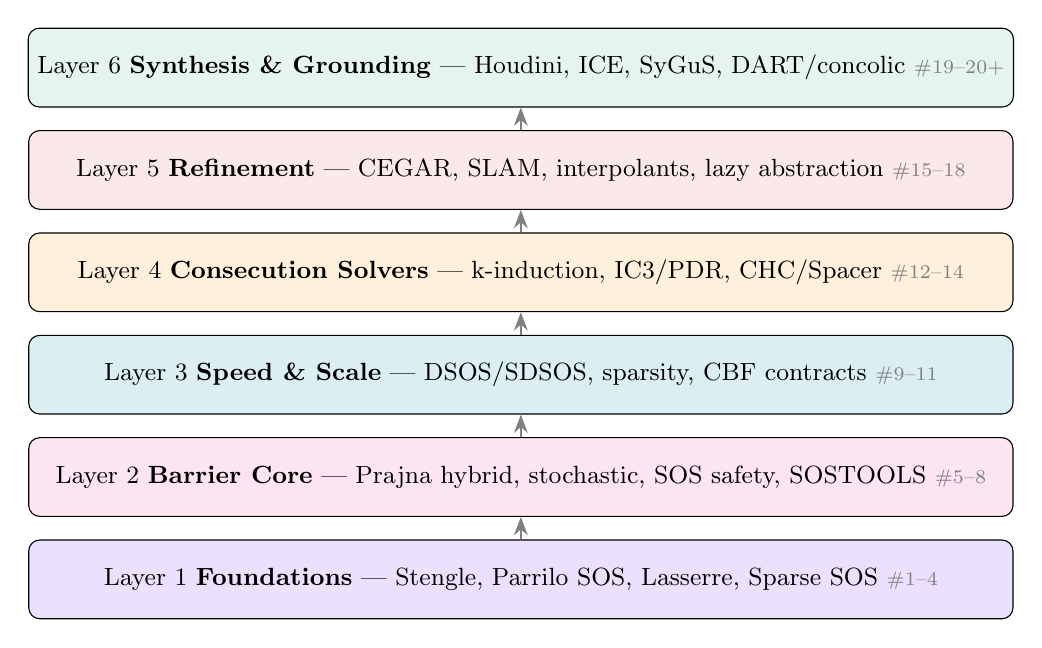
\begin{tikzpicture}[
  layer/.style={draw, rounded corners, minimum width=12.5cm, minimum height=1cm, align=center, font=\small},
]
  \node[layer, fill=hilbert!15] (l1) at (0,0) {Layer 1 \textbf{Foundations} --- Stengle, Parrilo SOS, Lasserre, Sparse SOS \hfill \textcolor{gray}{\scriptsize\#1--4}};
  \node[layer, fill=control!15] (l2) at (0,1.3) {Layer 2 \textbf{Barrier Core} --- Prajna hybrid, stochastic, SOS safety, SOSTOOLS \hfill \textcolor{gray}{\scriptsize\#5--8}};
  \node[layer, fill=verify!15] (l3) at (0,2.6) {Layer 3 \textbf{Speed \& Scale} --- DSOS/SDSOS, sparsity, CBF contracts \hfill \textcolor{gray}{\scriptsize\#9--11}};
  \node[layer, fill=steal!15] (l4) at (0,3.9) {Layer 4 \textbf{Consecution Solvers} --- k-induction, IC3/PDR, CHC/Spacer \hfill \textcolor{gray}{\scriptsize\#12--14}};
  \node[layer, fill=unsafe!10] (l5) at (0,5.2) {Layer 5 \textbf{Refinement} --- CEGAR, SLAM, interpolants, lazy abstraction \hfill \textcolor{gray}{\scriptsize\#15--18}};
  \node[layer, fill=safe!10] (l6) at (0,6.5) {Layer 6 \textbf{Synthesis \& Grounding} --- Houdini, ICE, SyGuS, DART/concolic \hfill \textcolor{gray}{\scriptsize\#19--20+}};

  \draw[-{Stealth}, thick, gray] (l1.north) -- (l2.south);
  \draw[-{Stealth}, thick, gray] (l2.north) -- (l3.south);
  \draw[-{Stealth}, thick, gray] (l3.north) -- (l4.south);
  \draw[-{Stealth}, thick, gray] (l4.north) -- (l5.south);
  \draw[-{Stealth}, thick, gray] (l5.north) -- (l6.south);
\end{tikzpicture}
\end{center}
\end{frame}

% ── Papers 1-4: Foundations ──────────────────────────────────────────────

\begin{frame}{\#1 Stengle 1974 --- Positivstellensatz}
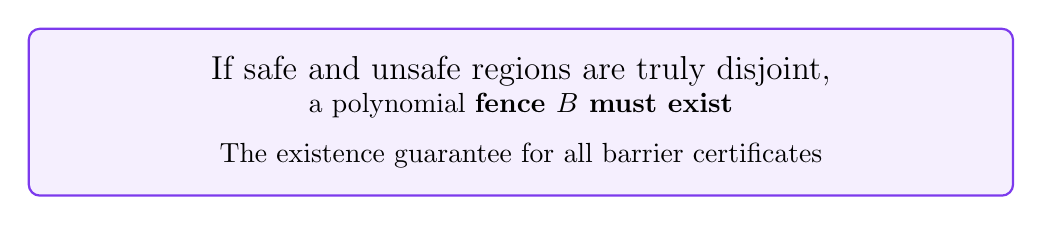
\begin{tikzpicture}
  \node[draw, rounded corners, fill=hilbert!8, thick, draw=hilbert, minimum width=12.5cm, align=center, inner sep=10pt] {
    \large If safe and unsafe regions are truly disjoint,\\a polynomial \textbf{fence $B$ must exist}\\[6pt]
    \normalsize The existence guarantee for all barrier certificates
  };
\end{tikzpicture}

\vspace{0.8em}
\textbf{Barrier role:} Theoretical bedrock. We \emph{know} a proof exists before we search for one.\\[3pt]
\textbf{How we bent it:} Map Python state variables $\to$ polynomial ring; interpret guards and error conditions as semialgebraic sets
\end{frame}

\begin{frame}{\#2 Parrilo 2000 --- SOS via SDP}
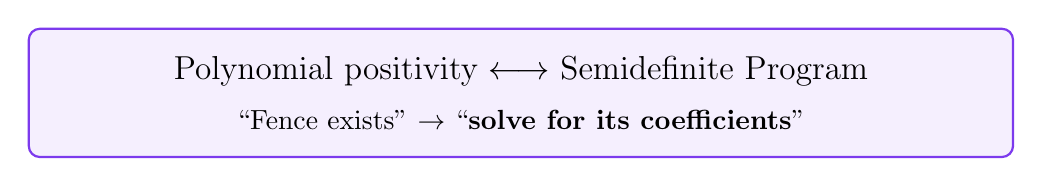
\begin{tikzpicture}
  \node[draw, rounded corners, fill=hilbert!8, thick, draw=hilbert, minimum width=12.5cm, align=center, inner sep=10pt] {
    \large Polynomial positivity $\longleftrightarrow$ Semidefinite Program\\[6pt]
    \normalsize ``Fence exists'' $\to$ ``\textbf{solve for its coefficients}''
  };
\end{tikzpicture}

\vspace{0.8em}
\textbf{Barrier role:} The computational engine for init and separation constraints.\\[3pt]
\textbf{How we bent it:} Parrilo's domain is Lyapunov for ODEs; we substitute the ODE state space with Python's symbolic machine state $\sigma$
\end{frame}

\begin{frame}{\#3 Lasserre 2001 --- Moment/SOS Hierarchy}

\begin{tikzpicture}
  \node[draw, rounded corners, fill=hilbert!8, thick, draw=hilbert, minimum width=12.5cm, align=center, inner sep=10pt] {
    \large Degree-$d$ certificate fails? Escalate to $d{+}2$\\[6pt]
    \normalsize Hierarchy \textbf{converges} --- systematic completeness
  };
\end{tikzpicture}

\vspace{0.8em}
\textbf{Barrier role:} Completeness ladder. No degree ceiling stops us permanently.\\[3pt]
\textbf{How we bent it:} Originally polynomial \emph{optimization}; we repurpose as \emph{feasibility-escalation} schedule --- each level is a portfolio tier, not an optimization step
\end{frame}

\begin{frame}{\#4 Sparse SOS (Waki et al., 2006)}
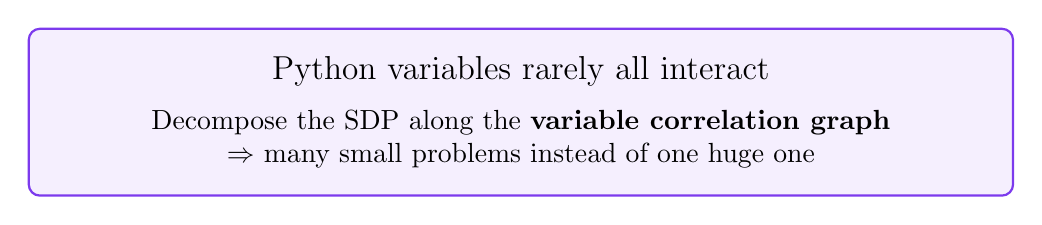
\begin{tikzpicture}
  \node[draw, rounded corners, fill=hilbert!8, thick, draw=hilbert, minimum width=12.5cm, align=center, inner sep=10pt] {
    \large Python variables rarely all interact\\[6pt]
    \normalsize Decompose the SDP along the \textbf{variable correlation graph}\\$\Rightarrow$ many small problems instead of one huge one
  };
\end{tikzpicture}

\vspace{0.8em}
\textbf{Barrier role:} Scalability for real functions with 10+ locals.\\[3pt]
\textbf{How we bent it:} Original graph from polynomial support; we build from Python \emph{data-flow} --- co-appearance in branch predicates or arithmetic
\end{frame}

% ── Papers 5-8: Barrier Core ────────────────────────────────────────────

\begin{frame}{\#5 Prajna \& Jadbabaie, HSCC 2004 --- Barrier Certificates}
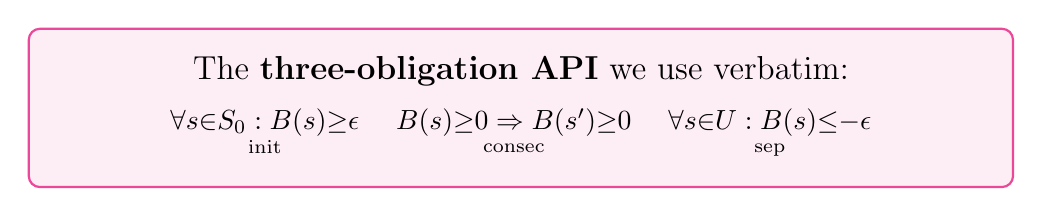
\begin{tikzpicture}
  \node[draw, rounded corners, fill=control!10, thick, draw=control, minimum width=12.5cm, align=center, inner sep=10pt] {
    \large The \textbf{three-obligation API} we use verbatim:\\[6pt]
    $\underset{\text{init}}{\forall s{\in}S_0: B(s){\ge}\epsilon}$
    \quad$\underset{\text{consec}}{B(s){\ge}0 \Rightarrow B(s'){\ge}0}$
    \quad$\underset{\text{sep}}{\forall s{\in}U: B(s){\le}{-}\epsilon}$
  };
\end{tikzpicture}

\vspace{0.8em}
\textbf{Barrier role:} \emph{The} paradigm. Every other paper serves these three conditions.\\[3pt]
\textbf{How we bent it:} Replace Lie-derivative consecution ($\dot{B} \ge 0$ along ODE flow) with symbolic one-step $B(\sigma') \ge 0$ under the discrete transition relation $T$
\end{frame}

\begin{frame}{\#6 Prajna et al., TAC 2007 --- Stochastic Barriers}

\begin{tikzpicture}
  \node[draw, rounded corners, fill=control!10, thick, draw=control, minimum width=12.5cm, align=center, inner sep=10pt] {
    \large Consecution as \textbf{expectation inequality}:\\[6pt]
    $\mathbb{E}[B(s') \mid s] \ge 0$ when $B(s) \ge 0$
  };
\end{tikzpicture}

\vspace{0.8em}
\textbf{Barrier role:} Extends barriers to non-deterministic/probabilistic transitions.\\[3pt]
\textbf{How we bent it:} Replace It\^{o} calculus over SDEs with Python probabilistic branching; expectation over path-condition probability mass
\end{frame}

\begin{frame}{\#7 SOS Safety Checker \quad\quad \#8 SOSTOOLS Framework}
\begin{columns}[c]
\begin{column}{0.48\textwidth}
\begin{block}{\#7: SOS Safety}
\begin{itemize}
  \item ``Can \emph{any} $B$ separate these regions?''
  \item Fast feasibility pre-check
  \item Skip expensive synthesis if no fence can exist
\end{itemize}
\end{block}
\end{column}
\begin{column}{0.48\textwidth}
\begin{block}{\#8: SOSTOOLS Engineering}
\begin{itemize}
  \item Configurable degree, variables
  \item Parametric template interface
  \item Production-grade solver plumbing
\end{itemize}
\end{block}
\end{column}
\end{columns}

\vspace{0.8em}
\centering\textbf{Role:} Make SOS synthesis \emph{practical} and configurable for CI throughput.
\end{frame}

% ── Papers 9-11: Speed & Scale ──────────────────────────────────────────

\begin{frame}{\#9 Ahmadi \& Majumdar, 2019 --- DSOS/SDSOS}
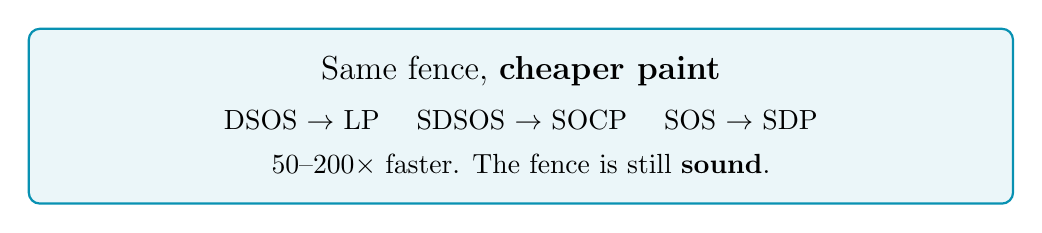
\begin{tikzpicture}
  \node[draw, rounded corners, fill=verify!8, thick, draw=verify, minimum width=12.5cm, align=center, inner sep=10pt] {
    \large Same fence, \textbf{cheaper paint}\\[6pt]
    \normalsize DSOS $\to$ LP \quad SDSOS $\to$ SOCP \quad SOS $\to$ SDP\\[4pt]
    50--200$\times$ faster. The fence is still \textbf{sound}.
  };
\end{tikzpicture}

\vspace{0.8em}
\textbf{Barrier role:} Speed tier. DSOS runs first; escalate to SOS only on failure.\\[3pt]
\textbf{How we bent it:} Originally robotics trajectory optimization; we discard the control objective and use it purely for certificate-existence checking
\end{frame}

\begin{frame}{\#10 CBF Survey (Ames et al., 2019)}
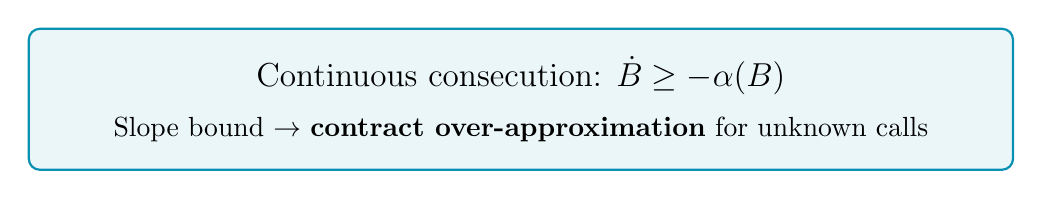
\begin{tikzpicture}
  \node[draw, rounded corners, fill=verify!8, thick, draw=verify, minimum width=12.5cm, align=center, inner sep=10pt] {
    \large Continuous consecution: $\dot{B} \ge -\alpha(B)$\\[6pt]
    \normalsize Slope bound $\to$ \textbf{contract over-approximation} for unknown calls
  };
\end{tikzpicture}

\vspace{0.8em}
\textbf{Barrier role:} Motivates how to handle library calls we can't analyze.\\[3pt]
\textbf{How we bent it:} Discretize the class-$\mathcal{K}$ slope bound into a per-call contract: $B(\sigma') \ge B(\sigma) - \alpha(B(\sigma))$ for black-box Python functions
\end{frame}

\begin{frame}{\#11 Correlative Sparsity in Practice}
\begin{center}
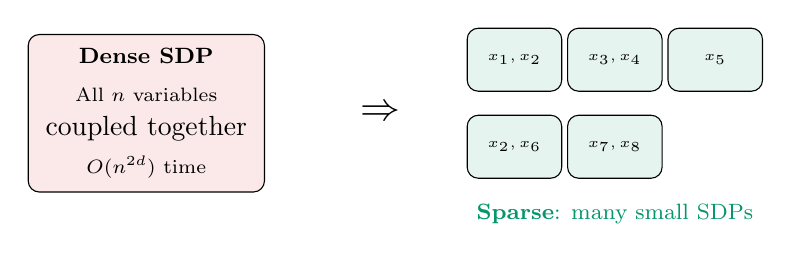
\begin{tikzpicture}[scale=0.85]
  % Dense SDP
  \node[draw, rounded corners, fill=unsafe!10, minimum width=3cm, minimum height=2cm, align=center] (dense) at (0,0) {
    \footnotesize\textbf{Dense SDP}\\[2pt]
    \scriptsize All $n$ variables\\coupled together\\[2pt]
    \scriptsize$O(n^{2d})$ time
  };

  \node[font=\Large] at (3.5,0) {$\Rightarrow$};

  % Sparse SDPs
  \node[draw, rounded corners, fill=safe!10, minimum width=1.2cm, minimum height=0.8cm, align=center, font=\tiny] at (5.5,0.8) {$x_1,x_2$};
  \node[draw, rounded corners, fill=safe!10, minimum width=1.2cm, minimum height=0.8cm, align=center, font=\tiny] at (7,0.8) {$x_3,x_4$};
  \node[draw, rounded corners, fill=safe!10, minimum width=1.2cm, minimum height=0.8cm, align=center, font=\tiny] at (8.5,0.8) {$x_5$};
  \node[draw, rounded corners, fill=safe!10, minimum width=1.2cm, minimum height=0.8cm, align=center, font=\tiny] at (5.5,-0.5) {$x_2,x_6$};
  \node[draw, rounded corners, fill=safe!10, minimum width=1.2cm, minimum height=0.8cm, align=center, font=\tiny] at (7,-0.5) {$x_7,x_8$};
  \node[font=\footnotesize, safe] at (7,-1.5) {\textbf{Sparse}: many small SDPs};
\end{tikzpicture}
\end{center}

\vspace{0.5em}
Variables in different branches rarely interact.\\
Sparsity makes barrier synthesis tractable for real Python functions.
\end{frame}

% ── Papers 12-14: Consecution Solvers ───────────────────────────────────

\begin{frame}{\#12 k-Induction (Sheeran et al., FMCAD 2000)}

\begin{tikzpicture}
  \node[draw, rounded corners, fill=steal!8, thick, draw=steal, minimum width=12.5cm, align=center, inner sep=10pt] {
    \large Does $B$ stay $\ge 0$ for $k$ steps, then \textbf{forever}?\\[6pt]
    \normalsize Bounded base + inductive step $\Rightarrow$ consecution proof
  };
\end{tikzpicture}

\vspace{0.8em}
\textbf{How we bent it:} Propositional SAT over hardware bit-vectors $\to$ SMT over integer/real program variables. Same base/step structure.
\end{frame}

\begin{frame}{\#13 IC3 (Bradley, VMCAI 2011)}
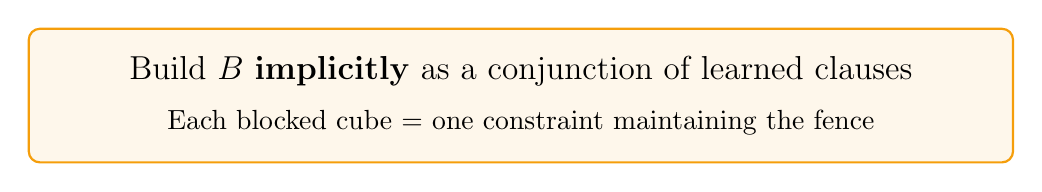
\begin{tikzpicture}
  \node[draw, rounded corners, fill=steal!8, thick, draw=steal, minimum width=12.5cm, align=center, inner sep=10pt] {
    \large Build $B$ \textbf{implicitly} as a conjunction of learned clauses\\[6pt]
    \normalsize Each blocked cube = one constraint maintaining the fence
  };
\end{tikzpicture}

\vspace{0.8em}
\textbf{How we bent it:} Boolean SAT over hardware registers $\to$ LIA predicates over Python state. Z3 model-based quantifier instantiation replaces SAT generalization.
\end{frame}

\begin{frame}{\#14 CHC/Spacer (Gurfinkel et al., CAV 2015)}
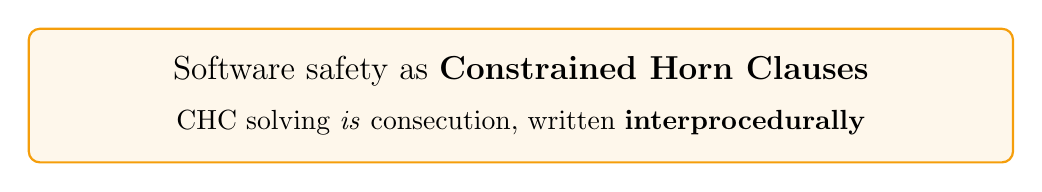
\begin{tikzpicture}
  \node[draw, rounded corners, fill=steal!8, thick, draw=steal, minimum width=12.5cm, align=center, inner sep=10pt] {
    \large Software safety as \textbf{Constrained Horn Clauses}\\[6pt]
    \normalsize CHC solving \emph{is} consecution, written \textbf{interprocedurally}
  };
\end{tikzpicture}

\vspace{0.8em}
\textbf{How we bent it:} SeaHorn targets C/LLVM; we re-encode for Python's transition system. Dynamic dispatch requires per-callsite CHC heads.
\end{frame}

% ── Papers 15-18: Refinement ────────────────────────────────────────────

\begin{frame}{\#15 CEGAR (Clarke et al., CAV 2000)}
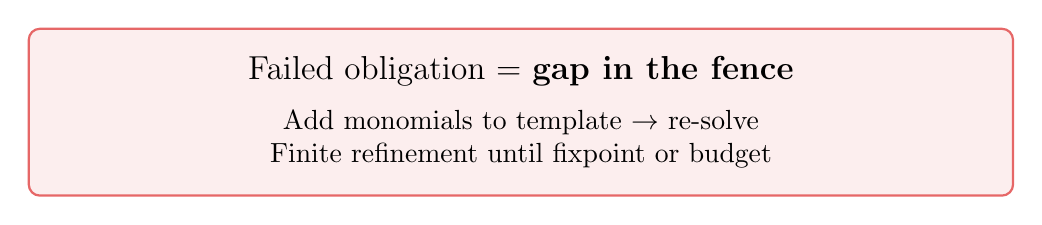
\begin{tikzpicture}
  \node[draw, rounded corners, fill=unsafe!8, thick, draw=unsafe!70, minimum width=12.5cm, align=center, inner sep=10pt] {
    \large Failed obligation = \textbf{gap in the fence}\\[6pt]
    \normalsize Add monomials to template $\to$ re-solve\\Finite refinement until fixpoint or budget
  };
\end{tikzpicture}

\vspace{0.8em}
\textbf{How we bent it:} Original ``abstraction'' is a boolean program; ours is the polynomial template degree and monomial basis
\end{frame}

\begin{frame}{\#16 SLAM (Ball et al., PLDI 2001)}
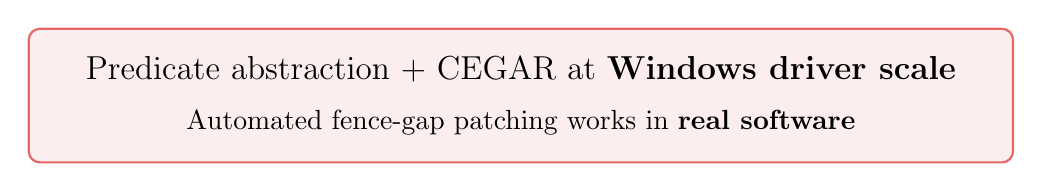
\begin{tikzpicture}
  \node[draw, rounded corners, fill=unsafe!8, thick, draw=unsafe!70, minimum width=12.5cm, align=center, inner sep=10pt] {
    \large Predicate abstraction + CEGAR at \textbf{Windows driver scale}\\[6pt]
    \normalsize Automated fence-gap patching works in \textbf{real software}
  };
\end{tikzpicture}

\vspace{0.8em}
\textbf{How we bent it:} We take the \emph{architectural} lesson and substitute a polynomial monomial selector for SLAM's boolean predicate engine
\end{frame}

\begin{frame}{\#17 Craig Interpolants (McMillan, CAV 2003)}
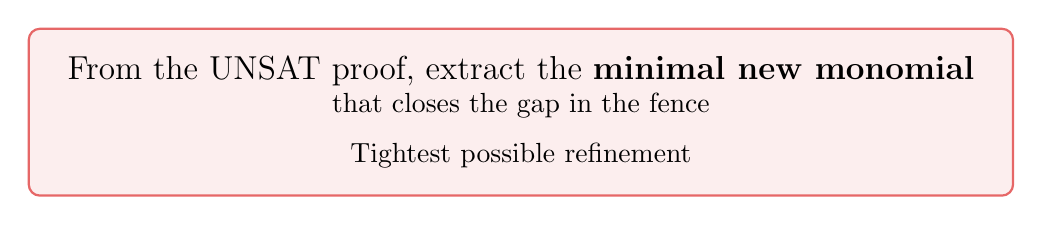
\begin{tikzpicture}
  \node[draw, rounded corners, fill=unsafe!8, thick, draw=unsafe!70, minimum width=12.5cm, align=center, inner sep=10pt] {
    \large From the UNSAT proof, extract the \textbf{minimal new monomial}\\that closes the gap in the fence\\[6pt]
    \normalsize Tightest possible refinement
  };
\end{tikzpicture}

\vspace{0.8em}
\textbf{How we bent it:} Original propositional/linear interpolants; we apply SMT interpolation over non-linear arithmetic
\end{frame}

\begin{frame}{\#18 Lazy Abstraction (Henzinger et al., POPL 2004)}
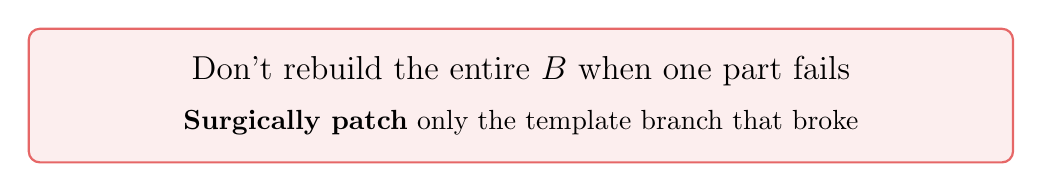
\begin{tikzpicture}
  \node[draw, rounded corners, fill=unsafe!8, thick, draw=unsafe!70, minimum width=12.5cm, align=center, inner sep=10pt] {
    \large Don't rebuild the entire $B$ when one part fails\\[6pt]
    \normalsize \textbf{Surgically patch} only the template branch that broke
  };
\end{tikzpicture}

\vspace{0.8em}
\textbf{How we bent it:} ``Subtree'' in BLAST is a CFG node set; in ours it's the monomial support region of $B$ around the failing check
\end{frame}

% ── Papers 19-20: Synthesis & Grounding ─────────────────────────────────

\begin{frame}{\#19 Houdini (Flanagan \& Leino, 2001) + ICE (Garg et al., 2014)}
\begin{columns}[c]
\begin{column}{0.48\textwidth}
\begin{block}{Houdini}
Start with many candidate coefficient configs.\\
Prune by counterexample.\\
Fixpoint = \textbf{widest valid $B$}.
\end{block}
\end{column}
\begin{column}{0.48\textwidth}
\begin{block}{ICE Learning}
Learn barrier from \textcolor{safe}{positive},\\
\textcolor{unsafe}{negative}, \textcolor{accent}{implication} examples.\\
Program's own behavior shapes $B$.
\end{block}
\end{column}
\end{columns}

\vspace{0.8em}
\textbf{How we bent them:} Houdini proposes boolean annotations for ESC/Java $\to$ we generate polynomial \emph{coefficient} candidates. ICE targets general first-order invariants $\to$ we restrict to bounded-degree polynomials.
\end{frame}

\begin{frame}{\#20 SyGuS (Alur et al., 2013) + DART/Concolic (Godefroid et al., 2005)}
\begin{columns}[c]
\begin{column}{0.48\textwidth}
\begin{block}{SyGuS}
Template family = grammar.\\
Three obligation checks = oracle.\\
Formalizes our coefficient search.
\end{block}
\end{column}
\begin{column}{0.48\textwidth}
\begin{block}{DART/Concolic}
Walk \textbf{real executions} to confirm\\$B \ge 0$ on live paths.\\Ground truth for the certificate.
\end{block}
\end{column}
\end{columns}

\vspace{0.8em}
\textbf{How we bent them:} SyGuS is generic (strings, bits, etc.) $\to$ we instantiate with a monomial grammar. DART's goal is \emph{falsification} $\to$ we \emph{invert} it to \emph{confirmation}.
\end{frame}

% ═══════════════════════════════════════════════════════════════════════════
%  ACT V — CONTRACTS + BARRIERS
% ═══════════════════════════════════════════════════════════════════════════

\begin{frame}[fragile]{Contracts: How PyTorch Meets Barriers}
\begin{center}
\textbf{Problem:} the analyzer hits \texttt{torch.cosine\_similarity()} --- what is the output?
\end{center}

\vspace{0.5em}
\begin{columns}[T]
\begin{column}{0.52\textwidth}
\begin{lstlisting}[language=Python]
sim = torch.cosine_similarity(x, y)
score = sim - 3
result = 1.0 / score  # DIV_ZERO?
\end{lstlisting}

\vspace{0.3em}
\textbf{Without contract:} \texttt{sim} is unknown $\to$ FP.

\vspace{0.3em}
\textbf{With contract:} \texttt{sim} $\in [-1, 1]$\\
$\Rightarrow$ \texttt{score} $\in [-4, -2]$\\
$\Rightarrow$ $0 \notin [-4, -2]$\\
$\Rightarrow$ \textcolor{safe}{\textbf{Division is provably safe.}}
\end{column}
\begin{column}{0.43\textwidth}
\centering
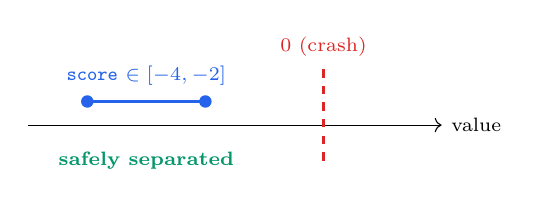
\begin{tikzpicture}[scale=0.75]
  \draw[->] (-5,0) -- (2,0) node[right,font=\scriptsize]{value};
  \draw[very thick, accent] (-4,0.4) -- (-2,0.4);
  \fill[accent] (-4,0.4) circle (3pt);
  \fill[accent] (-2,0.4) circle (3pt);
  \node[above, font=\scriptsize, accent] at (-3,0.5) {\texttt{score} $\in [-4,-2]$};
  \draw[very thick, unsafe, dashed] (0,-0.6) -- (0,1);
  \node[above, font=\scriptsize, unsafe] at (0,1) {$0$ (crash)};
  \node[font=\scriptsize, safe] at (-3,-0.6) {\textbf{safely separated}};
\end{tikzpicture}
\end{column}
\end{columns}
\end{frame}

\begin{frame}{Contracts Are Barrier Constraints on Library Outputs}
\begin{center}
\begin{tikzpicture}[
  box/.style={draw, rounded corners, fill=white, minimum width=3.5cm, minimum height=1.3cm, align=center, font=\small, thick}
]
  \node[box, draw=control] (contract) at (0,0) {
    \textbf{Contract}\\[2pt]
    \texttt{cos\_sim} $\in [-1,1]$
  };
  \node[box, draw=accent] (interval) at (5,0) {
    \textbf{Interval algebra}\\[2pt]
    \texttt{score} $\in [-4,-2]$
  };
  \node[box, draw=safe] (barrier) at (10,0) {
    \textbf{Barrier check}\\[2pt]
    $0 \notin [-4,-2]$ \;\textcolor{safe}{\faCheck}
  };

  \draw[-{Stealth}, very thick] (contract) -- (interval);
  \draw[-{Stealth}, very thick] (interval) -- (barrier);
\end{tikzpicture}
\end{center}

\vspace{0.8em}
\textbf{Soundness:} $\text{Sem}_f \subseteq R_f$ (contract over-approximates actual behavior).\\[3pt]
\textbf{Consecution with contracts:}
\[
B(s) \ge 0 \;\wedge\; T_{\text{prog}}(s,s') \;\wedge\; C_{\text{library}}(s,s') \;\Rightarrow\; B(s') \ge 0
\]

\vspace{0.3em}
Better contracts $\to$ tighter intervals $\to$ more bugs proven unreachable $\to$ less noise.
\end{frame}

\begin{frame}{PyTorch Contract Examples}
\begin{center}
\renewcommand{\arraystretch}{1.3}
\begin{tabular}{llll}
\toprule
\textbf{Function} & \textbf{Output bounds} & \textbf{Precondition} & \textbf{Barrier effect} \\
\midrule
\texttt{torch.rand(*size)} & $[0, 1)$ & --- & excludes $<0$ from downstream \\
\texttt{torch.zeros(*size)} & $= 0$ & --- & known constant \\
\texttt{torch.eye(n)} & $[0, 1]$ & --- & bounded outputs \\
\texttt{torch.arange(s,e,st)} & $[s, e{-}st]$ & $st \neq 0$ & \textbf{flags DIV\_ZERO if $st=0$} \\
\texttt{cos\_similarity} & $[-1, 1]$ & --- & tight interval propagation \\
\texttt{view(*shape)} & shape-preserving & $\prod = $ numel & \textbf{shape safety} \\
\bottomrule
\end{tabular}
\end{center}

\vspace{0.5em}
1{,}500+ lines of PyTorch contracts. Each one is a barrier constraint on library outputs that composes through interval algebra.
\end{frame}

% ═══════════════════════════════════════════════════════════════════════════
%  ACT VI — FINAL NOTES
% ═══════════════════════════════════════════════════════════════════════════

\begin{frame}{What Actually Shipped}
\begin{center}
\texttt{pip install a3-python}
\end{center}

\vspace{0.5em}
\begin{columns}[T]
\begin{column}{0.48\textwidth}
\begin{block}{Static stage (bulk)}
\begin{itemize}
  \item Bytecode analysis + Z3
  \item Barrier certificate proofs
  \item 67 bug types
  \item \textbf{99\% eliminated}
\end{itemize}
\end{block}
\end{column}
\begin{column}{0.48\textwidth}
\begin{block}{Agentic stage (residue)}
\begin{itemize}
  \item Multi-turn LLM tool-use
  \item Reads files, searches guards
  \item Zero API keys in CI
  \item Handles the $\sim$1\%
\end{itemize}
\end{block}
\end{column}
\end{columns}

\vspace{0.5em}
\centering
\textbf{Proof artifacts are upstream. LLM judgment is downstream.}
\end{frame}

\begin{frame}{The Meta-Lesson}
\begin{center}
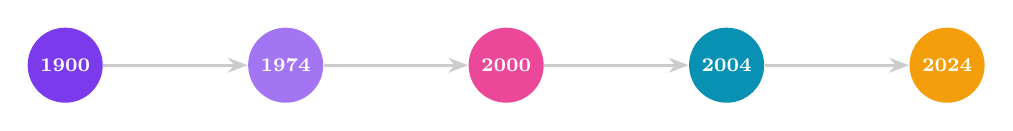
\begin{tikzpicture}[
  dot/.style={circle, minimum size=9mm, draw=none, font=\scriptsize\bfseries, text=white},
  conn/.style={-{Stealth[length=2.5mm]}, very thick}
]
  \node[dot, fill=hilbert] (d1) at (0,0) {1900};
  \node[dot, fill=hilbert!70] (d2) at (2.8,0) {1974};
  \node[dot, fill=control] (d3) at (5.6,0) {2000};
  \node[dot, fill=verify] (d4) at (8.4,0) {2004};
  \node[dot, fill=steal] (d5) at (11.2,0) {2024};

  \draw[conn, gray!40] (d1) -- (d2);
  \draw[conn, gray!40] (d2) -- (d3);
  \draw[conn, gray!40] (d3) -- (d4);
  \draw[conn, gray!40] (d4) -- (d5);
\end{tikzpicture}
\end{center}

\vspace{1em}
\begin{enumerate}
  \item \textbf{Hilbert} asked if non-negative polynomials are sums of squares (1900)
  \item \textbf{Stengle} proved polynomial infeasibility has algebraic certificates (1974)
  \item \textbf{Parrilo} made this computable with SDPs --- for \emph{control theory} (2000)
  \item \textbf{Prajna} wrote three barrier obligations --- for \emph{verification} (2004)
  \item \textbf{We} stole 20 techniques, bent them into those three obligations, and applied them to \emph{Python bytecode} (2024--2026)
\end{enumerate}

\vspace{0.5em}
\centering
\large\textbf{The dots were always there. We just drew the line.}
\end{frame}

\begin{frame}[standout]
\Large Questions?

\vspace{1em}
\normalsize
\texttt{pip install a3-python}\\[4pt]
\texttt{a3 scan . --triage}\\[12pt]
\small From Hilbert's 17th Problem to your CI pipeline.
\end{frame}

\end{document}
